% !TeX root = main.tex
\section{不同模型与数据条件下的策略求解}\label{sec:solving}

长期准则确定后，求解方法取决于能获得哪些环境信息。模型可用时，可以直接预测候选决策的后果；允许交互时，可以持续采样并更新价值函数、环境模型或策略；只有固定历史数据时，估计与优化都只能依靠已有记录。

本章前三节按这三类信息条件讨论针对单一给定偏好的求解方法，每节内部按第~\ref{sec:criteria}~章的准则类型排列：线性或阶段可加准则、非线性 SER、非线性 ESR、优先级与约束。第~\ref{sec:solving-reuse}~节集中讨论在多个给定偏好之间复用计算和数据的方法，第~\ref{sec:solving-summary}~节总结准则、信息条件与方法之间的对应。模型使用方式和数据获取方式是两个交叉的维度：模型可以来自机理知识，也可以从在线或离线数据中学习，规划同样可以建立在近似模型上。因此，这里的划分刻画的是方法所依赖的信息，而不是互斥的算法范式。

图~\ref{fig:solver-taxonomy}~按信息条件概括代表性求解机制，为本章的方法讨论提供导航；准则与适用条件的详细对应见表~\ref{tab:solver-routes}。

\begin{figure}[H]
\centering
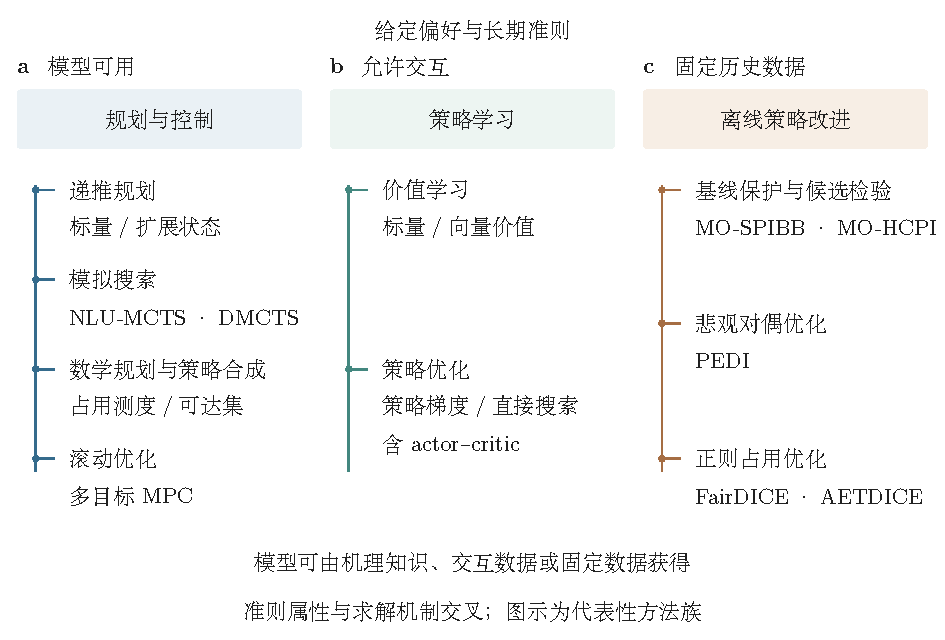
\includegraphics{figures/solver_taxonomy.pdf}
\caption{不同信息条件下的代表性求解机制。三组对应第~\ref{sec:solving-model}--\ref{sec:solving-offline}~节，允许交叉组合，且不构成穷尽分类。MO-SPIBB 与 MO-HCPI 分别采用基线保护约束和候选策略的统计检验\cite{satija2021mospibb}；PEDI 结合对偶更新与悲观估计\cite{wu2021pedi}；FairDICE 与 AETDICE 优化带分布正则项的占用测度，后者在增广状态中处理累计结果变换\cite{kim2025fairdice,kim2026aetdice}。AETDICE 为预印本方法，具体准则和保证条件见正文。}
\label{fig:solver-taxonomy}
\end{figure}

\subsection{模型可用条件下的规划与控制}\label{sec:solving-model}

模型可用时，可以依据状态转移和回报机制预测候选决策的长期影响。显式动力学方程便于构造递推关系、约束条件和数值优化问题；只提供轨迹生成能力的模拟器则适合通过搜索或抽样估计候选策略的长期表现。两种情形下，求解过程都要保留第~\ref{sec:structure}~章所要求的状态信息、价值表示和策略类别。

对于固定线性偏好，或本身就是阶段效用累积的准则，状态满足 Markov 条件时可以直接采用标量动态规划或相应的控制方法。这类规划得到的是执行时根据状态作出反应的闭环策略，与只优化一条固定动作序列的开环规划不同。

累计结果上的非线性 ESR 要求规划保留已实现的结果。NLU-MCTS 将实际执行中已累计的回报与树内搜索及随机 rollout 获得的未来回报按同一折扣基准相加，再对完整结果施加效用函数；反向传播的是这一完整结果的效用，候选动作的期望效用由访问计数估计\cite{hayes2023}。DMCTS 在同一评价结构下维护期望效用的 bootstrap 近似后验，并用 Thompson 采样选择搜索动作。两种方法分别以上置信探索和后验采样分配模拟预算，评价对象都是原 ESR；DMCTS 的后验描述的是期望效用估计的不确定性，并不保存完整的多维回报分布。它们需要能够反复模拟后续过程的模型，搜索预算、rollout 策略和模型误差共同决定最终的动作选择。

扩展状态上的近似动态规划给出了另一条路线。Peng 等在有限状态、有限动作、确定有界向量回报及一致连续效用下，以累计回报网格近似扩展状态，利用连续模 $\delta_\epsilon$ 将回报近似误差转化为效用误差\cite{peng2025esr}：若 $\|\mathbf x-\mathbf y\|_1<\delta_\epsilon$ 时有 $|u(\mathbf x)-u(\mathbf y)|<\epsilon$，有限时域近似动态规划达到 $\epsilon$ 最优，计算复杂度为
\begin{equation}
O\!\left(|\mathcal S|^2|\mathcal A|\left(\frac{mT^2}{\delta_\epsilon}\right)^m\right).
\end{equation}
目标维数以指数方式进入网格规模，时域和精度要求也会抬高代价，无限折扣时域还需额外控制截断误差。这说明，恢复递推结构并不等于求解代价低。一致连续性不要求效用可微，但排除了不连续的阈值效用。

优先级规划通过逐层限制后续决策来保留严格优先关系，而不依赖一个足够大的补偿权重。Wray 等的 LMDP 允许为不同状态分区规定不同的目标顺序，每一级价值迭代完成后，只把相应 $Q$ 值距最优值不超过局部容差的动作传给下一目标\cite{wray2015lmdp}。在无限折扣问题中，局部容差 $\eta_i=(1-\gamma)\delta_i$ 控制其向长期允许损失 $\delta_i$ 的累积；不同分区之间存在循环依赖时，整体收敛还依赖论文给出的分区条件。容差为零与允许高优先级目标让步，对应的是两种不同的决策要求。

部分可观测情形下，同样的思路转移到信念空间。LPOMDP 对所有信念使用同一优先顺序，先按高优先级价值限制每个信念下的可行动作，再进行低优先级备份\cite{wray2015lpomdp}。精确 LVI 保留相应的 $\alpha$ 向量组合，LPBVI 只在采样信念上更新以减少计算。近似价值误差会影响哪些动作被保留或删除，因此需要与容差预算一起处理。

概率阈值和长期平均要求可以直接写成策略合成查询。Brázdil 等用线性约束刻画长期平均多目标问题的可达回报集合，并构造实现相应结果的策略\cite{brazdil2014}。Forejt 等将多目标可达概率与期望总奖励约束化为一系列加权问题：每次求得策略后记录其各目标表现，再用分离超平面选择下一组权重，从内外两侧逼近可达结果集合\cite{forejt2012pareto}。这种查询既能判断给定阈值是否可实现，也能近似给出取舍边界；有限时界要求通过相应时域的价值迭代处理，无界奖励则要求奖励有限并满足相应的符号条件。

Quatmann 和 Katoen 进一步把期望长期平均奖励与期望总奖励的组合纳入多目标模型检验，并扩展到包含连续时间行为的 Markov 自动机\cite{quatmann2021longrun}。算法在允许策略随机化的可达集合上维护
\begin{equation}
\operatorname{downconv}(\mathcal P)\subseteq\mathcal C\subseteq
\bigcap_j\{\mathbf x:\mathbf w_j^\top\mathbf x\leq v_j\},
\end{equation}
其中 $\mathcal P$ 是已实现的期望结果向量，$\mathcal C$ 为逐分量向下闭的可达集合，$v_j$ 是相应加权问题的上界。目标阈值落入内部集合即可实现，超出外部界即不可实现，介于两者之间时继续细化。求解加权子问题时，长期平均部分利用最大端分量内的长期行为，并在商模型中与总奖励部分衔接。该分析要求各目标的上确界有限，混合总奖励还要求端分量内符号一致；它处理的是多个期望准则，不涉及 ESR 或逐轨迹同时达标。

对于具有显式动力学和约束的任务，模型预测控制通过重复求解有限预测时域问题并执行当前动作，实现滚动优化与反馈控制。多目标情形不仅要求得 Pareto 控制序列，还要规定相邻时刻如何在这些序列中选择。设系统动力学为 $x_{t+1}=f(x_t,u_t)$，目标 $i$ 的阶段成本和终端代价分别为 $\ell_i$ 和 $F_i$。Grüne 和 Stieler 的一种构造使用共同的局部终端反馈 $\kappa$，要求每个终端代价满足 $F_i(f(x,\kappa(x)))+\ell_i(x,\kappa(x))\leq F_i(x)$，并在下一时刻选择不劣于移位延续序列的候选解\cite{gruene2019}。在终端不变性、相关 Pareto 集的外部稳定性等条件下，该机制保持可行性，并得到各目标闭环成本上界
\begin{equation}
J_i^\infty(x_0,\mu_N)
\leq J_i^N(x_0,\mathbf u_0^\star),\qquad \forall i,
\end{equation}
其中 $\mu_N$ 是滚动优化形成的闭环控制律，右侧为初始所选预测控制序列的含终端代价成本。Pareto 集的外部稳定性指每个可行成本向量都存在逐分量不劣的 Pareto 向量。若阶段成本之和相对于共同平衡点正定，闭环轨迹还会收敛。这些闭环性质来自选择规则与终端设计的配合；在预测时域内任选一个 Pareto 解得不到这些性质，也不等于原偏好下的无限时域最优策略。

显式多目标 MPC 把重复优化的主要计算移到运行之前。Bemporad 和 Muñoz de la Peña 针对线性动力学，将特定凸分段仿射代价或一个二次目标与其余分段仿射目标的控制问题写成多参数规划，预先构造关于状态和目标权重的分段仿射控制解\cite{bemporad2009mompc}。在线选择权重时还须满足由上一时刻移位序列形成的价值下降约束，稳定性依赖各目标的正定性、共同终端反馈和终端不变性。该方法允许目标权重随状态变化，但为维持稳定可能修正权重，因此实际执行的控制律与最初希望表达的取舍会有差别。

在非线性系统中，Hernández Castellanos 等针对初始状态不确定构建离线控制序列库，利用问题对称性减少需预计算的参数维数，在线阶段插值获得候选，再用参考点优化修正控制序列\cite{hernandez2020explicit}。这一机制把大规模前沿搜索放在离线阶段，在线只针对当前给定偏好做局部求解，修正阶段同时处理不确定性与可行约束。论文的实验针对规定的初始条件不确定集合和汽车机动仿真。

模型方法的实际表现还取决于模型质量、预测时域和数值求解精度。模型偏差影响动作后果的估计，有限预测时域截断远期影响，数值优化引入近似误差；对于数据驱动模型，策略还可能偏向模型误差较大的状态区域。因此，这类方法需要同时报告模型预测性能和闭环策略表现，并说明预测时域、终端价值、约束软化和模型近似各自的作用。

\subsection{允许环境交互条件下的策略学习}\label{sec:solving-online}

准确模型未知但允许交互时，可以用新增的状态、动作和回报样本学习价值函数、环境模型或参数化策略。固定线性偏好与期望可加回报下，先将回报标量化，再采用单目标学习方法即可。需要保留多个目标的信息时，可以学习向量价值，在动作选择或策略更新阶段再引入给定偏好。策略梯度、策略搜索和进化优化则直接以完整策略为优化对象，不依赖局部 Bellman 分解，但要面对长期回报估计方差、探索效率和约束满足等问题\cite{hayes2022}。无论采用哪种表示，学习目标都要与 SER、ESR、优先级或约束结构对应。

非线性 SER 的策略更新需要在整体期望结果处计算目标取舍。设参数化策略为 $\pi_\theta$，固定初始状态分布下的期望累计回报向量为 $\mathbf v(\theta)=\mathbb E_{\pi_\theta}[\mathbf G]$。当效用与期望回报均可微时，由链式法则得
\begin{equation}
\nabla_\theta u_p(\mathbf v(\theta))
=\sum_{i=1}^{m}
\partial_i u_p(\mathbf v(\theta))\,
\nabla_\theta v_i(\theta).
\end{equation}
因此，可以分别估计各目标的策略梯度，再用当前期望结果处的边际效用组合更新方向。这些系数随策略表现变化，计算位置也不同于对每一步即时回报施加非线性效用。Agarwal 等将这一机制用于非线性多目标学习，为每个目标配置 critic 估计价值和优势\cite{agarwal2022nonlinear}。该研究的理论对象是凹、Lipschitz 效用作用于长期平均回报向量的问题：模型方法通过后验采样获得转移模型，在占用测度流约束下求解凹效用最大化，学习保证依赖有限状态动作、有限直径及平稳策略诱导的不可约性；深度 actor--critic 版本则由实验支持。

这类更新还隐含一种不同于回报方差的估计误差。即使 $\widehat{\mathbf v}$ 是期望回报的无偏估计，代入非线性边际效用后，$\mathbb E[\partial_i u_p(\widehat{\mathbf v})]$ 一般也不等于 $\partial_i u_p(\mathbf v)$。Ganesh 和 Aggarwal 的 2026 年预印本针对折扣凹 SER，用多层 Monte Carlo 估计控制这一代入偏差，并结合自然策略梯度更新\cite{ganesh2026bias}。在奖励有界、效用偏导 Lipschitz、策略对数梯度有界且 Lipschitz、Fisher 信息矩阵一致正定等条件下，论文得到 $\widetilde O(\epsilon^{-2})$ 的期望样本复杂度，平均效用差中仍含策略类与兼容函数逼近造成的误差项；若效用满足相应的二阶平滑条件，普通自然策略梯度也能达到同阶结果。由此看，非线性 SER 的样本效率同时受效用平滑性和策略表示条件影响，而不只取决于各目标价值估计的精度。

凹 SER 还可以放到一般效用强化学习的框架中理解。定义折扣占用测度
\begin{equation}
\lambda^\pi(s,a)=\mathbb E_\pi\!\left[\sum_{t\geq0}\gamma^t\mathbf1_{\{S_t=s,A_t=a\}}\right].
\end{equation}
各目标的期望回报是 $\lambda^\pi$ 的线性函数，凹效用 $u(\mathbf v^\pi)$ 因而可以写成占用测度上的凹泛函 $F(\lambda^\pi)$。Zhang 等通过效用的 Fenchel 对偶，将相应策略梯度的估计转化为随机鞍点问题，并利用占用测度中的隐藏凸性分析策略搜索\cite{zhang2020general}。在有限状态动作、初始分布全支持，以及占用测度映射、逆映射和平滑性满足相应条件时，精确梯度迭代具有全局性能收敛界。Barakat 等进一步建立一般凹效用下的梯度支配关系，并通过最大似然估计占用测度，使估计复杂度与所用函数类的参数维数相关\cite{barakat2025general}。其大规模离散问题分析要求占用测度可实现、策略得分及效用梯度有界且平滑，以及参数化保持占用测度的局部可逆结构；可实现性不成立时会留下函数逼近误差。两项工作的全局保证都来自期望回报或占用测度中的结构，而不是策略梯度本身。

公平性准则是非线性 SER 的具体例子。Siddique 等采用广义 Gini 福利函数：先将各目标的期望回报从小到大排序，再以递减的正权重加权，使较差目标获得更大的边际关注\cite{siddique2020fair}。其策略梯度方法根据当前期望回报的排序组合各目标梯度。论文同时指出，所构造的 GGF-DQN 更新实际优化的是期望中的 Gini 评价下界，与期望结果上的评价并不相同，两种算法之间的差别在于随机性的处理方式，而不只是福利函数本身。

若给定准则直接要求改善最差目标，则问题为
\begin{equation}
\max_\pi\min_{1\leq i\leq m}v_i^\pi
=\max_{\lambda\in\mathcal D}\min_{\mathbf w\in\Delta_m}
\sum_{i=1}^m w_i\sum_{s,a}\lambda(s,a)r_i(s,a),
\end{equation}
其中 $\mathcal D$ 是满足折扣流平衡条件的非负占用测度集合。Park 等利用这一结构构造线性规划及其对偶，并以熵正则化消除从对偶最优权重恢复策略时的歧义\cite{park2024maxmin}：只求出一个最优权重、再任选该权重下的确定性最优动作，可能得到最差目标表现为零的策略，最大最小准则仍可能需要随机化。Byeon 等将正则化问题写成策略学习者与目标权重对手之间的零和博弈，以自然策略梯度和镜像下降构成单循环更新\cite{byeon2025maxmin}。其最后迭代收敛分析针对表格 softmax 策略、规定的正则化和步长，近似评价会留下与评价误差相关的邻域，深度 PPO 及自适应正则化版本由实验支持。这里学习到的权重是固定 max-min 准则的求解变量，不是从数据中推断的用户偏好。

多目标梯度方法的保证对象也各不相同。Zhou 等的 MOAC 通过估计共同改进方向，给出折扣和平均回报情形下的有限时间 Pareto 驻点分析\cite{zhou2024moac}。Pareto 驻点表示不存在各目标共同改善的局部方向，与前述凹效用的全局性能界、max-min 正则化博弈的收敛对象含义不同，也不说明某个给定效用已达到全局最优。

非线性 ESR 的学习需要反映效用作用于累计结果这一特点。Reymond 等用多维回报分布构造 critic，把未来回报与已累计结果一起代入效用函数，形成与 ESR 对应的策略更新\cite{reymond2023}。后续研究把分布价值表示用于具体任务，例如基础设施维护中成本与风险的权衡\cite{remmerden2025}。这类方法的关键在于价值表示能提供计算长期效用所需的信息，是否需要完整回报分布取决于具体准则。它与 SER 在均值向量处组合梯度的机制不同：在非线性效用下，逐轨迹结果及其相依关系会影响期望效用。

Cai 等给出另一种保留完整累计效用的在线求解方式\cite{cai2023dpmorl}。在有限时域、$\gamma>0$ 时，把累计回报 $\mathbf c_t$ 和时间加入状态，并构造增量奖励
\begin{equation}
\rho_t=\gamma^{-t}\bigl[u(\mathbf c_{t+1})-u(\mathbf c_t)\bigr],
\qquad
\sum_{t=0}^{T-1}\gamma^t\rho_t=u(\mathbf c_T)-u(\mathbf0).
\end{equation}
右侧与原完整结果效用只差一个常数，因此在扩展信息可用时，标量奖励学习器就能优化原 ESR。等价变换本身不保证 PPO 或 SAC 找到全局最优策略。其 DPMORL 框架还生成多样的单调效用函数并分别训练策略，为分布偏好保留候选，但有限个效用并不覆盖全部单调效用。

词典序学习需要在优化低优先级目标时保住高优先级表现。Skalse 等的价值学习方法按优先级逐层缩小可选动作集合，只保留 $Q$ 值距当前最优值不超过容差的动作，后续目标的备份和选择都限制在这一集合内\cite{skalse2022}。表格收敛结果要求有限状态动作、有界奖励、折扣因子小于 $1$ 或几乎必然终止、所有状态动作对被无限访问，学习率满足随机逼近条件，且容差小于相关非零价值间隙。策略梯度版本通过不同时间尺度的更新和高优先级性能约束实现分层优化。容差、价值估计误差与更新尺度共同决定优先级能否保住，表格情形的收敛结果不覆盖深度函数逼近。期望累计成本约束则把可接受性作为独立的可行域处理，例如 Achiam 等的约束策略优化\cite{achiam2017}，它与词典序的逐层排序承担不同作用。

Abdolmaleki 等的 MO-MPO 在动作分布空间组织多目标更新\cite{abdolmaleki2020mompo}。它为每个目标构造相对于当前策略受 KL 限制的改善动作分布，再通过监督拟合合成单一参数化策略，每个目标允许的 KL 变化量表示其对更新的相对影响。这一接口减弱了奖励尺度对偏好设置的影响，但 KL 参数并不对应某个预先给定效用中的权重。用 MO-MPO 求解给定的效用、阈值或风险要求时，需要说明接口与原准则如何对应，并按原准则评价结果；动作分布的融合也不提供 ESR 所需的累计结果信息。

允许交互的好处是可以主动采集新的决策数据，改善对相关状态与动作的估计；代价是探索本身消耗时间、资源，并可能带来安全风险。对于有安全约束的任务，训练阶段的约束违反和最终部署策略的约束表现应分别记录\cite{skalse2022,achiam2017}。训练主要在仿真器中进行时，还要区分仿真样本效率与真实系统的数据成本；若学习过程同时估计模型并据此规划，实际采集的数据与模型生成的数据也应分开说明。

\subsection{固定历史数据条件下的策略学习}\label{sec:solving-offline}

离线条件下，策略只能用预先收集的历史数据训练，无法通过新的交互验证或补充当前策略所需的信息。离线求解首先要回答两个问题：数据记录了哪些变量，行为策略覆盖了哪些状态、动作和长期结果。

第一个问题决定数据能否重建原长期准则。数据保存了原始多维回报时，只要环境机制与目标定义不变，就可以按任意固定权重重新构造标量回报；若只保存了某一历史权重下的标量奖励，各目标分量已被压缩，可分析的偏好范围随之受限。阶段效用累积需要逐阶段回报，或足以恢复阶段效用的信息；累计结果上的非线性 ESR 需要轨迹关联信息，至少要能重建累计量、事件和约束；非线性 SER 则需要据此估计候选策略的期望回报向量。

第二个问题决定策略估计的可靠性。候选策略频繁选择数据中很少出现的动作时，其价值估计主要依赖函数逼近和分布外外推。单目标离线强化学习常用保守价值估计、行为约束或不确定性建模控制外推误差\cite{kumar2020}；多目标问题还需要明确这些机制保护的是加权总价值、各目标表现，还是原有的可接受性条件。较强的行为约束限制了外推，也限制了策略超越历史行为的空间；偏好变化则会改变需要改进的行为区域。

线性偏好下，可以显式限制离线改进的幅度，使各目标都不差于基线。MO-SPIBB 在有限状态动作、有界奖励及已知行为基线 $\pi_b$ 的条件下优化正线性权重下的价值，并要求策略在估计不确定性较大的动作上接近基线\cite{satija2021mospibb}。其 Soft-SPIBB 约束为 $\sum_a e(s,a)|\pi(a\mid s)-\pi_b(a\mid s)|\leq\epsilon$，其中 $e(s,a)$ 是由日志数据得到的误差界；算法还加入各目标的基线优势约束，并在每个状态求解线性规划。在概率至少为 $1-\delta$ 的估计事件上，各目标真实价值满足
\begin{equation}
V_i^\pi(s)-V_i^{\pi_b}(s)
\geq-\frac{\epsilon V_{\max}}{1-\gamma},\qquad i=1,\ldots,m,
\end{equation}
其中 $V_{\max}$ 为价值幅度上界。这是一种允许统计误差的逐目标基线保护，并非逐条轨迹的物理安全保证。同一研究中的 MO-HCPI 使用独立的训练与安全检验数据，通过各目标的重要性加权下置信界联合筛选候选策略。两者分别代表优化约束和事后统计检验两条路径。

非线性 SER 与期望结果约束可以通过对偶化和悲观估计共同处理。PEDI 研究有限时域成本问题 $\min_\pi g(\mathbf V^\pi_1)$，并要求期望累计成本向量位于给定目标集内\cite{wu2021pedi}。其中 $g$ 为凸、逐坐标单调不减且 Lipschitz 的函数，目标集为满足几何 Slater 条件的非空闭凸下集。算法利用凸共轭把非线性成本和目标集距离惩罚转化为一系列线性成本问题，交替执行对偶变量更新与悲观价值迭代；由于目标是成本最小化，悲观性体现为在成本估计中加入不确定性惩罚。最终策略在每次执行开始时随机选取一个迭代策略并全程执行，以实现迭代价值的平均。性能差距与约束违反界都含有沿最优策略轨迹累积的数据不确定性，因此不要求全空间统一覆盖，但最优行为的支持不足时误差界会很大。这些保证针对期望成本。

占用测度优化提供了处理非线性长期效用的另一条路径。FairDICE 将各目标期望回报的严格凹福利总和与相对于数据占用分布的 $f$ 散度正则化共同优化，并以占用流约束保证策略一致性\cite{kim2025fairdice}。其对偶变量对应当前福利目标的边际取舍；在最优对偶权重处，正则化非线性问题与相应的正则化线性问题等价。这里的权重由已给定福利函数的优化产生，不是学习到的决策者偏好。AETDICE 将评价形式扩展为 $\mathcal G(\mathbb E[\mathcal F(\mathbf G^\pi)])$，在有限时域中把已累计回报与时间加入状态，利用变换 $\mathcal F$ 的增量奖励建立占用测度优化，从而覆盖 SER、ESR 及其组合\cite{kim2026aetdice}。外层 $\mathcal G$ 为线性时，可以得到与相应可加目标的等价表示；一般分析还依赖外层凹性、变换平滑性及正则项的严格凸性。该方法要求数据在每个可达的增广状态、动作和时刻上具有正占用密度，这比普通状态动作上的支持要求更强。

上述方法分别用逐目标基线保护、悲观对偶优化和占用测度正则化控制离线改进，优化对象和保证范围各不相同。约束、尾部风险和达标概率需要与原准则匹配的估计，主目标上的保守性推不出它们的表现。离线求解前应分别检查两件事：数据能否重建长期准则，以及数据是否覆盖目标策略的决策区域。这两项条件互不替代，增加同类样本也无法弥补记录内容的缺失。

\subsection{跨偏好的计算与数据复用}\label{sec:solving-reuse}

偏好在求解时已经给定，但不同偏好之间仍可以共享数据和计算。常见的组织方式有三种：针对当前偏好独立求解；预先构建覆盖多种偏好的候选策略集合；训练以偏好或目标结果为条件输入的统一策略。三种方式都能服务于给定偏好决策，区别在于训练成本、表示范围和泛化要求\cite{vamplew2011}。本节按信息条件介绍后两种方式，最后讨论非线性效用下的候选覆盖。

图~\ref{fig:preference-reuse}~对照了三种方式从给定偏好到执行策略的接口与共享对象。

\begin{figure}[H]
\centering
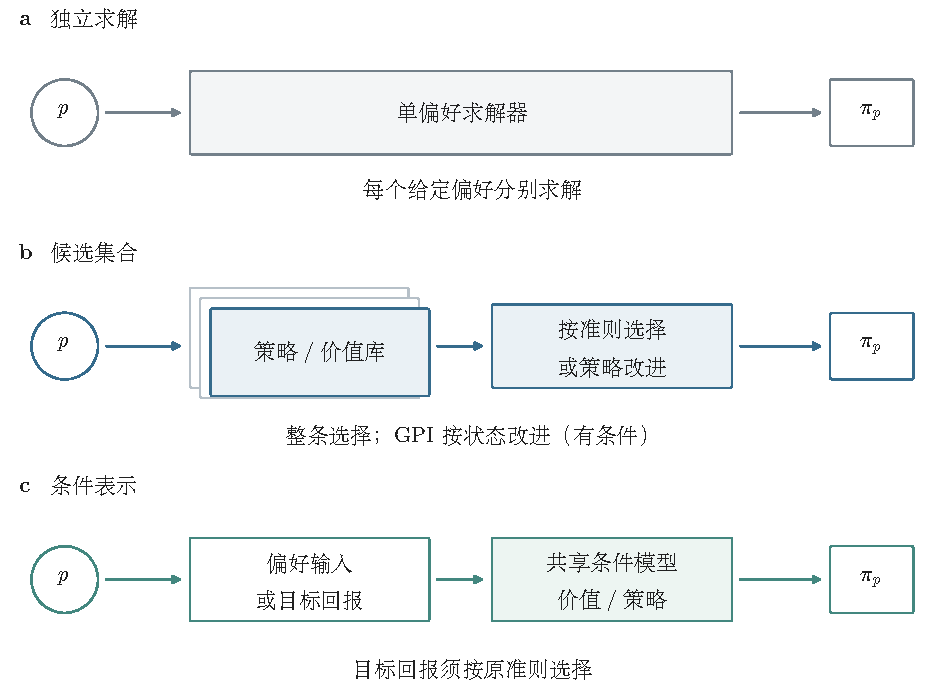
\includegraphics{figures/preference_reuse.pdf}
\caption{面向多个给定偏好的求解组织方式。独立求解为每个偏好分别计算策略；候选集合复用已有策略及其评价；条件表示共享模型参数。整条策略选择与逐状态的广义策略改进（GPI）不同，后者的性能性质依赖回报结构与评价精度等条件\cite{barreto2017sf}。条件价值需经动作选择形成策略；目标回报条件模型须先按原准则确定目标，不能把目标回报等同于偏好权重\cite{reymond2022pcn,zhu2023}。三种组织方式可以组合，图中不比较性能或计算成本。}
\label{fig:preference-reuse}
\end{figure}

\subsubsection{模型可用时的候选集合规划}

共享多个线性偏好的规划可以在算法内部或外部组织。内部方法直接把标量价值替换为候选向量集合：凸包价值迭代（CHVI）在状态动作对上保留对某个线性权重最优的向量，通过后继集合的加权组合与凸包剪枝完成备份\cite{barrett2008}。与保留全部 Pareto 向量相比，它只保存线性偏好所需的凸覆盖信息。

环境随机时，候选集合的递推要组合不同后继状态上的后续选择。Chen 等以有限状态动作、非负成本的多目标随机最短路径问题为例，采用向量集合价值迭代，并通过启发式搜索减少需要更新的状态\cite{chen2023mossp}。设 $\mathcal V_k(s)$ 表示状态 $s$ 的候选期望成本向量集合，其更新可写为
\begin{equation}
\begin{aligned}
\mathcal Q_{k+1}(s,a)
&=\{\mathbf c(s,a)\}\oplus
\bigoplus_{s'}P(s'\mid s,a)\mathcal V_k(s'),\\
\mathcal V_{k+1}(s)
&=\operatorname{CCS}\!\left(\bigcup_a\mathcal Q_{k+1}(s,a)\right),
\end{aligned}
\end{equation}
其中 $\oplus$ 为向量集合的 Minkowski 和，$\operatorname{CCS}$ 保留支持线性成本权衡的凸覆盖信息。这里采用到达目标即终止的无折扣成本，目标状态 $g$ 的终端集合为 $\mathcal V_k(g)=\{\mathbf 0\}$。不同后继状态可以对应不同的后续决策，因此期望运算需要组合各后继状态的候选向量。MOLAO* 在部分解图上扩展状态并更新其祖先，MOLRTDP 通过试运行和残差检查逐步标记已求解状态，二者都要处理多个不可比较的候选动作。收敛分析要求适当的可达性条件和可采纳启发式，并需排除不能以概率 $1$ 到达目标的策略；论文用适当策略成本的已知向量上界识别这类不适当策略。这些结果针对线性成本权衡下的凸覆盖。

集合值递推还要保证组合出来的尾部选择能由允许的策略实现。Mifrani 对 White 的早期向量 Bellman 扩展给出有限时域反例：分别从不同后继状态选取候选尾部价值并求加权和，所得向量未必对应同一条确定性 Markov 策略，因为不同分支随后汇合时，可能要求该策略在同一状态与时刻采取不同动作\cite{mifrani2025bellman}。在该研究的模型中，确定性转移，或允许策略利用已达状态的历史，可以恢复集合方程的可实现性。CON-MODP 处理的正是这一问题：它同时存储价值与策略，对只在当前扩展状态出现冲突的候选强制采用同一动作并重新评价，其收敛结果针对确定性转移的无限时域折扣多目标 MDP\cite{wiering2007conmodp}。因此，对向量价值集合做备份时，除了数值上的支配关系，还要说明集合覆盖的策略类别，以及后继策略的组合是否仍属于该类别。

精确剪枝通常需要反复求解线性规划，检验某一候选是否存在能使其优于其余候选的权重或信念。BLP 利用相邻价值迭代中这些线性规划的相似性，把上一轮相似问题中决定最优解的约束映射到当前候选集合作为初始约束，再逐步加入违反的约束，直到完成原问题的检查\cite{roijers2018bootstrap}。它减少的是重复求解的工作量，剪枝检验本身照常完成，这与直接截断候选集合、以覆盖精度换速度的近似机制不同。

外部方法保留单目标求解器，通过选择权重逐步构建覆盖。AOLS 利用当前标量化价值包络的分片线性凸结构，在潜在改进较大的角点权重处调用求解器，并根据新增向量重新计算角点与误差界\cite{roijers2014aols}。底层求解器具有已知的相对近似保证时，该误差可以用来构造近似凸覆盖；底层若只是没有误差证书的启发式规划器，就得不到同样的覆盖保证。对于给定偏好问题，这类多偏好规划的作用是预先复用计算；如果只需处理一个固定偏好，应比较额外覆盖成本与直接求解的成本。

不完全观测会改变规划所需的状态。对于转移与观测模型已知的多目标 POMDP，OLSAR 将单目标 POMDP 的 $\alpha$ 向量扩展为保留各目标价值的 $\alpha$ 矩阵；给定信念 $b$ 和权重 $\mathbf w$，候选矩阵 $A$ 的标量价值为 $b^{\mathsf T}A\mathbf w$\cite{roijers2015olsar}。外层乐观线性支持依据当前凸覆盖的潜在改进选择待求解权重，内层点基规划用先前得到的矩阵初始化价值下界，从而避免从头规划，也减少额外的策略评价。近似覆盖保证继承底层标量 POMDP 求解器的误差；采用点基方法时，该误差还取决于采样信念对信念空间的覆盖密度，矩阵复用本身主要改善计算时间。与 OLSAR 按线性权重构建覆盖不同，第~\ref{sec:solving-model}~节的 LPOMDP 在信念空间中共享的是保持优先级的动作限制，两者不能通过更换权重输入相互替代。

\subsubsection{交互学习中的策略库与条件策略}

策略库方法首先共享已有策略及其评价。Natarajan 和 Tadepalli 在加权平均回报问题中缓存有限个策略及其向量评价，新权重给定后选择已有策略继续改进\cite{natarajan2005}。DOL 将外循环乐观线性支持与向量输出的深度 Q 学习结合，比较了复用全部网络参数与只保留特征层、重新训练输出层两种做法\cite{mossalam2016dol}。复用收益来自已有表示对后续偏好求解的初始化；神经子求解器的近似误差会进入覆盖结果，外循环的理论性质并不延伸到深度训练过程。

策略集合需要解决多个候选价值如何共同学习，以及执行时如何恢复所选策略。Pareto Q-learning 将即时回报的均值与后续非支配价值集合分开保存，避免在不断变化的两个向量集合之间建立不稳定的一一更新关系\cite{vanmoffaert2014pql}。确定性转移下，动作价值集合由即时均值加上折扣后的后继候选集合构成；随机转移扩展则按观测到的转移频率组合不同后继状态的向量集合。学习阶段可以用超体积、集合基数或支配关系引导探索；执行阶段则要先选定一个目标期望回报向量并持续跟踪对应策略，而不是在每个状态任选一个局部非支配动作。该方法针对回合式任务学习确定性非平稳候选策略，论文没有给出正式的收敛证明，其价值集合也不是 ESR 所需的回报分布表示。

在共享动力学、只有回报权衡变化的任务中，后继特征为复用提供了显式分解。若条件期望即时回报满足 $r_{\mathbf w}(s,a,s')=\boldsymbol\phi(s,a,s')^\top\mathbf w$，则
\begin{equation}
\begin{aligned}
Q_{\mathbf w}^{\pi}(s,a)
&=\boldsymbol\psi^\pi(s,a)^\top\mathbf w,\\
\boldsymbol\psi^\pi(s,a)
&=\mathbb E_\pi\!\left[\sum_{t\geq0}\gamma^t\boldsymbol\phi(S_t,A_t,S_{t+1})\mid S_0=s,A_0=a\right].
\end{aligned}
\end{equation}
Barreto 等据此在新权重下直接重评既有策略，再进行广义策略改进\cite{barreto2017sf}。Borsa 等的通用后继特征近似进一步把策略的任务编码作为条件输入，使价值表示能在已学策略之间泛化\cite{borsa2019usfa}。前者复用回报权重，后者复用策略表示，两者都以共享动力学、线性回报表示和足够准确的评价为前提。

给定新偏好后，广义策略改进（GPI）用当前权重评价库 $\Pi$ 中每个策略的向量动作价值，再在动作和策略两个维度上选择：
\begin{equation}
\pi_{\mathrm{GPI}}(s;\mathbf w)
\in\arg\max_a\max_{\pi\in\Pi}
\mathbf w^{\mathsf T}\mathbf Q^\pi(s,a).
\end{equation}
在固定线性偏好、折扣可加回报及准确策略评价下，所得策略至少不劣于库中任一策略\cite{alegre2026}。与整条选用库中某个策略不同，改进策略可以逐状态利用不同候选策略的后续价值。Alegre 等进一步以 GPI 能带来的价值改进决定训练哪些权重，并用相应误差确定生成和使用模型样本的优先级。GPI-LS 的覆盖保证要求单偏好求解器达到最优或规定的近似精度；GPI-PD 学习下一状态与完整向量奖励的联合模型，使同一模型服务于多个权重；其不确定性感知扩展用价值估计的置信下界抑制高估动作，在下界有效时给出相对于库中最好策略的性能余量。这些保证建立在线性组合、候选覆盖和估计误差之上。

多个偏好也可以作为相关子问题，在策略群体中共享搜索信息。MORL/D 将偏好采样、经验池、邻域协作、策略改进与外部档案组织为可组合的求解框架\cite{felten2024decomposition}。PGMORL 维护策略群体，依据历史改进数据预测不同训练方向的收益，选择策略和权重继续训练，并通过 Pareto 分析和插值扩展候选\cite{xu2020pgmorl}。与每个权重从头训练相比，这些方法把计算分配和经验共享纳入复用机制，其覆盖质量和插值效果由实验评估，没有给定偏好下的效用误差保证。

连续候选集也可以不以偏好权重为输入。Parisi 等学习从低维变量到策略参数的流形，使其在目标空间中的像逼近 Pareto 前沿\cite{parisi2016manifold}；后续工作在每次执行开始时探索策略参数，并以重要性采样复用历史执行数据\cite{parisi2017reuse}。使用时仍需依据原效用在流形可表示的候选中选择，前沿质量指标的优化也不等同于对每个给定效用取得最优。

条件价值网络则用一个网络代替显式存储的策略集合。Abels 等把线性权重作为多目标价值网络的输入\cite{abels2019}，Envelope 方法更新时在当前权重下同时比较不同动作和其他权重对应的候选向量价值\cite{yang2019}：更新下一状态价值时，选择使 $\mathbf w^{\mathsf T}Q(s',a',\mathbf w')$ 最大的候选向量，而不只在当前权重 $\mathbf w$ 下搜索动作，再把该向量与即时向量回报组成更新目标。这样，其他偏好下已探索到的折中结果也能用于当前偏好的学习。作者在有界价值、折扣因子小于 $1$ 的理想更新设定中，以各权重的标量化价值定义伪距离并分析固定点；实际的深度网络通过有限偏好采样、向量误差与标量化误差的联合训练近似这一更新，理想算子的收敛结论不覆盖这一训练过程。

近期研究进一步处理条件网络中的共享表示和训练冲突。COLA 用与目标无关的潜在动力学表示共享转移知识，并在不同偏好的价值更新发生冲突时限制相互干扰\cite{li2025cola}。$D^3$PO 公开稿分别计算逐目标优势和 PPO 裁剪损失，再按偏好加权，并用动作分布差异正则化抑制条件策略的行为塌缩\cite{ambadkar2026d3po}。Chen 等从无奖励强化学习出发，把其训练目标作为辅助任务，并结合偏好引导探索，以改善不同偏好之间的知识共享\cite{chen2026rewardfree}；训练阶段为多个潜在查询收集可复用信息，回答查询时偏好仍是给定输入，相关实验以 MO-Gymnasium 基准和消融设置检验辅助任务与探索策略的作用。这些工作都在连续控制或标准基准上检验机制，没有给出非线性效用下的覆盖保证。

样本重用方式会改变条件网络实际学到的偏好范围。Bonin 等的近期公开稿研究了以已实现结果方向替换请求偏好的回溯重标记，发现在所测的离策略连续控制任务中，该机制可能使训练集中到少数已访问的偏好区域，并提出混合保留原请求偏好的修正\cite{bonin2026collapse}。结论限于所测算法、目标数和任务；它的启示是，应检查样本复用是否持续覆盖需要回答的偏好查询，而不是只看数据被重复使用的次数。

条件策略中的“偏好一致”也可能指不同的目标。PCRL 将输入参数解释为期望回报方向，通过目标梯度与方向相似性梯度共同更新\cite{yang2025pcrl}。其理论分析给出平滑性、梯度估计及步长等条件下的 Pareto 驻点和相似性驻点，论文也指出驻点未必具有高相似度。回报方向接近输入参数，与最大化同一参数所定义的线性加权效用，是两种需要分别评价的选择规则。

目标回报条件策略提供了不同于价值递推的共享路径。Pareto Conditioned Networks（PCN）把状态、目标剩余回报向量及剩余时域作为输入，把轨迹中实际采取的动作作为监督标签，通过动作分类训练一个能够复现不同结果的网络\cite{reymond2022pcn}。每条新轨迹按各时刻的实际后续回报重新标注；训练期间，算法从已有非支配结果附近提出改进目标，继续与环境交互，并保留不同结果区域的轨迹以维持覆盖。因此，PCN 虽然使用监督更新，整体仍包含主动采集轨迹。部署时输入的是目标结果而非效用权重，要服务于给定偏好，还需依据原效用或可接受性规则选定希望实现的结果，并检验条件策略的实际表现。实验展示了单个网络覆盖非凸折中区域的能力，论文没有给出任意目标回报可达或任意非线性效用最优的理论结论。Vamplew 等的 steering 方法同样以目标点组织非平稳策略学习，并与平稳确定性策略进行实验比较\cite{vamplew2017steering}。这类目标点接口都需要与给定效用或可接受性规则相连；本文只讨论目标已经给定时的求解接口，不讨论用户在学习过程中修改目标的情形。

\subsubsection{固定数据下的偏好复用}

固定数据下，多个偏好可以共享同一批轨迹。Lizotte 等在有限时域、无折扣的多奖励批量学习中，以线性函数拟合各动作的价值，并在权重单纯形上保留分片线性表示\cite{lizotte2012}。在特征矩阵满列秩且采用无正则最小二乘时，省略动作下标，某一阶段的回归系数可写为
\begin{equation}
\widehat{\boldsymbol\beta}_t(\mathbf w)
=(\Phi_t^{\mathsf T}\Phi_t)^{-1}\Phi_t^{\mathsf T}\widehat{\mathbf y}_t(\mathbf w),
\qquad
\widehat y_{t,n}(\mathbf w)
=\mathbf w^{\mathsf T}\mathbf r_{t,n}
+\widehat V_{t+1}(s_{t+1,n},\mathbf w),
\end{equation}
其中 $\Phi_t$ 是特征矩阵，$n$ 标识历史样本。终端阶段可以线性组合各基奖励的拟合系数；此前阶段的最优动作随权重变化，回归目标需要依据各样本的权重分区共同细分，三目标情形则通过单纯形三角剖分组织这些分片。这种复用依赖回归与价值包络的结构，分片数会随时域和目标维数增长，只训练偏好端点再插值得不到全部策略。

MOFQI 不显式维护单纯形上的分片，而是把固定偏好参数作为价值函数的输入。它将单目标拟合 $Q$ 迭代扩展到状态、动作与线性权重的联合空间，在一次训练中共享不同权重下的回归\cite{castelletti2012mofqi,castelletti2013water}。在成本最小化记号下，备份仍针对同一权重计算后续价值，即以 $\mathbf w^{\mathsf T}\mathbf c+\gamma\min_{a'}\widehat Q_{k-1}(s',a',\mathbf w)$ 构造回归目标；同一环境转移可以配上多个采样权重，但权重在一次序贯问题中保持不变。与解析保留分片相比，树回归直接逼近连续偏好域，减轻了显式分区的存储负担，精度则取决于样本、权重采样和函数逼近。

对于带偏好标签的多目标示范，PEDA 以偏好和向量剩余回报为条件，通过 Decision Transformer 或回报条件监督学习生成动作\cite{zhu2023}。训练数据按各目标尺度归一化，动作损失拟合历史轨迹中的行为；部署时要给出与当前偏好匹配、且数据能够支持的目标回报。D4MORL 中不同数据质量与偏好覆盖的设置显示了这些信息条件的影响；其实验指标依据行为策略的参考前沿计算，并不代表相对真实最优前沿的性能。若示范的偏好没有记录，直接模仿全部轨迹会把相互冲突的取舍混进同一行为正则项。PRMORL 用归一化轨迹回报近似行为偏好，根据它与给定权重的相似度筛选示范，并结合表达能力更强的生成策略及偏好条件价值学习\cite{lin2024offline}。这一标签推断只用于筛选历史数据，当前决策者给定的偏好仍是优化输入；轨迹回报提供的是启发式标签。该方法在部署时调整行为正则化强度的阶段使用了新采集的环境轨迹，这部分适应成本应与固定数据训练分开计算。

偏好条件生成方法以轨迹片段为建模对象。MODULI 以偏好和回报为条件生成状态序列，再用逆动力学模型恢复待执行动作；它对目标回报做偏好相关的归一化，并学习沿偏好变化方向调整去噪过程的适配器，把生成从数据覆盖区域引向未覆盖的偏好区域\cite{yuan2025moduli}。DiffMORL 同样采用偏好条件扩散规划，但主要通过离线数据混合增强训练样本，改善对未见偏好的生成表现\cite{xiao2025diffmorl}。前者调整生成时的条件引导，后者增强训练数据，两者都不同于 PEDA 直接监督拟合历史动作。D4MORL 实验支持它们在所测偏好分布上的泛化表现；生成轨迹和扩充的条件标签仍需由实际动力学与回报支持，生成能力本身说明不了未覆盖偏好下的最优性或可行性。

偏好条件方法复用的是数据中已有的行为，不会增加数据中没有观察到的动作后果。因此，第~\ref{sec:solving-offline}~节关于记录内容和数据覆盖的两项检查同样适用于这里，而且需要针对每个待回答的偏好分别进行。

\subsubsection{非线性效用下的候选覆盖}

线性权重下的凸覆盖只保留了均值信息。非线性 ESR 下，Röpke 等研究了多维回报分布之间的支配关系，以及它与期望效用和 Pareto 支配之间的联系\cite{ropke2023}。其分布支配以联合累积分布函数的排序为基础，并要求至少一个目标的边缘分布严格改善。相应的分布未支配集（distributional undominated set，DUS）保留不被其他候选分布支配的策略，它包含期望回报的 Pareto 前沿，也可能保留在期望意义下受支配的策略。凸分布未支配集（convex distributional undominated set，CDUS）进一步检查其他回报分布的混合能否支配某一候选，以缩小集合规模。

这类剪枝的效用保证有明确的范围。该研究对两维回报证明：对于严格单调且满足 $\partial^2u/\partial x_1\partial x_2\leq0$ 的效用，分布支配意味着更高的期望效用，混合支配则保证至少有一个组成分布优于被支配的候选。该交叉导数条件描述的是目标联合取值的偏好结构，与效用的凹性是两回事。联合分布还保留了目标间的依赖；用边缘累积分布函数的乘积代替联合分布，只有在目标独立时才有相应的支配解释。计算中，回报被投影为有限类别分布，使支配检查能在有限支持点上进行；分布精度与候选集合规模都会增加存储和计算代价，额外的集合截断也可能丢掉需要的候选\cite{ropke2023}。因此，只依据期望回报向量筛选 ESR 候选可能丢失有价值的策略，而分布表示与剪枝规则也必须和具体的效用类别相匹配。

对于明确给定的非线性效用族，已有工作直接以原准则性能定义覆盖。Kim 等针对广义 $p$-mean 福利函数，把 max-min、几何平均与算术平均纳入 $p\in[-\infty,1]$ 的同一参数族，并分别给出 SER 和 ESR 两种聚合\cite{kim2025portfolio}。在有限状态动作、固定起点与固定有限时域、逐阶段各目标奖励严格正有界 $0<L\leq r_i\leq U$，且能在同一可行策略集合 $\Pi$ 内求出每个参数 $p$ 下最优策略的条件下，其算法自适应选择参数，构造对整个族都具有 $\alpha$ 乘法近似保证的策略组合；记 $\kappa=U/L$，组合规模上界为 $O(\log\kappa/\log(1/\alpha))$。相邻参数热启动分析还控制了已有最优策略在新参数下的福利损失。这里的组合是供不同效用选择的候选集合，执行时不需要随机混合；用启发式求解器替代最优 oracle 后，近似保证需要相对于该求解器重新解释。这一结果说明，跨偏好复用可以围绕明确的效用族建立性能保证，而不只依靠前沿几何指标描述覆盖。第~\ref{sec:solving-online}~节 DPMORL 生成的多样单调效用也服务于同一目的，但没有相应的覆盖保证。

\subsubsection{复用方法的适用范围}

上述方法共享数据、表示和计算的方式不同：显式价值集合保留多个可比较的结果，条件价值网络共享各偏好下的估计，GPI 利用候选策略的价值做逐状态改进，目标回报条件网络则共享已实现结果与动作之间的映射。策略的组织形式需要与偏好类别、可搜索的策略类别以及数据支持范围相对应。

复用方法的有效范围由训练时覆盖的偏好形式和参数区域决定。线性权重下的凸覆盖和均值信息、非线性 SER 在受限策略类别下的候选保留要求、非线性 ESR 的分布信息要求，三者需要分别分析；允许策略混合时，可达期望回报集合也会改变。参考点、词典序和硬约束可能要求不同的条件输入、排序机制和可接受性检查，只修改一个权重标签并不能让原有网络覆盖这些问题。针对单一偏好的专门求解可以集中模型容量和采样资源；复用方法的收益则应通过覆盖误差、新偏好的追加求解成本和部署计算量来衡量，而不只看平均解集指标。

最后，在不同任务之间切换偏好，与在同一执行过程中改变偏好是两类问题。前者是多个给定偏好问题之间的策略复用；后者会影响已实现累计结果的解释，并可能改变整个长期决策准则。本文关注求解或部署开始时已经确定的偏好，因此把跨偏好方法视为数据与计算的复用机制，不展开偏好获取和执行中偏好变化的问题。

\subsection{结构条件与求解路线的对应}\label{sec:solving-summary}

综合第~\ref{sec:structure}~章的结构分析与本章的方法，求解路线可以按“长期准则---信息表示---策略类别---模型与数据条件”的顺序组织。长期准则决定评价什么，状态与价值表示决定保留哪些信息，策略类别限定可搜索的决策规则，模型与数据条件决定这些信息从何处获得。

表~\ref{tab:solver-routes}~汇总上述对应关系。可等价转化的期望可加准则允许直接调用标量方法；非线性 SER 围绕期望向量或占用测度组织优化，非线性累计结果 ESR 则需保留足以计算完整结果效用的信息。词典序、期望约束和路径概率要求还须保留各自的比较次序或可接受性条件，不能相互代替。实际任务中的这些结构可以组合，具体方法的保证仍以相应的效用、策略、模型和数据假设为前提。

\begin{table}[H]
\centering
\caption{长期准则与模型、数据条件下的求解路线}
\label{tab:solver-routes}
\begingroup
\zihao{5}\songti
\setlength{\tabcolsep}{5pt}
\renewcommand{\arraystretch}{1.18}
\setlength{\reviewtablewidth}{\dimexpr\textwidth-6\tabcolsep\relax}
\begin{tabular}{@{}P{0.25\reviewtablewidth}P{0.25\reviewtablewidth}P{0.25\reviewtablewidth}P{0.25\reviewtablewidth}@{}}
\toprule
准则与关键信息 & 模型可用 & 允许交互 & 固定历史数据 \\
\midrule
期望可加标量准则\newline 固定取舍、Markov 信息 & 标量动态规划\cite{hayes2022}\newline 转移与回报模型 & 标量回报学习\cite{hayes2022}\newline 探索与采样条件 & 重标奖励后学习\cite{zhu2023}\newline 原始回报与行为支持 \\
\addlinespace[7pt]
非线性 SER\newline 期望向量、策略随机化 & 凹效用占用优化\cite{zhang2020general}\newline 有限状态动作等条件 & 整体期望处组合梯度\cite{agarwal2022nonlinear}\newline 区分理论与深度实现 & FairDICE\cite{kim2025fairdice}\newline 凹福利的正则占用优化 \\
\addlinespace[7pt]
非线性累计结果 ESR\newline 累计量、时间、效用信息 & 扩展状态近似规划\cite{peng2025esr}\newline 有限模型、连续效用；或模拟搜索\cite{hayes2023} & 累计状态与效用增量\cite{cai2023dpmorl}\newline 有限时域下保持目标 & AETDICE\cite{kim2026aetdice}\newline 增广状态上的正则优化与数据支持 \\
\addlinespace[7pt]
优先关系\newline 次序、容差、估计误差 & LMDP 逐层限动作\cite{wray2015lmdp}\newline 容差与分区条件 & 词典序价值或策略更新\cite{skalse2022}\newline 充分访问、适当容差 & 本文未作\newline 专门方法比较 \\
\addlinespace[7pt]
期望结果约束\newline 目标、可行域、随机化 & 约束查询与可达集逼近\cite{forejt2012pareto} & CPO\cite{achiam2017}\newline 期望成本约束下的策略更新 & PEDI\cite{wu2021pedi}\newline 凸成本、目标集及数据支持 \\
\addlinespace[7pt]
路径概率或联合达标\newline 事件、记忆、联合信息 & 概率性质合成\cite{etessami2008modelchecking}\newline 可能需记忆与随机化 & 按指定事件评价和更新；本文未作专门比较 & 事件可恢复、策略有支持；均值保护不等于概率保证 \\
\bottomrule
\end{tabular}
\par\vspace{4pt}\raggedright\noindent
注：各行可组合，信息条件也可交叉；完整条件见第~\ref{sec:solving-model}--\ref{sec:solving-offline}~节。标量化仍须匹配时间结构并保留独立约束；ESR 近似规划中的效用要求一致连续。FairDICE、AETDICE 含分布散度正则，AETDICE 为预印本。未列专门方法不表示该方向不存在方法。
\par\endgroup
\end{table}


当多个给定偏好需要依次求解时，第~\ref{sec:solving-reuse}~节的复用方法可以分摊计算和数据成本，但其保证范围受偏好类别、候选覆盖和估计误差的限制。求得策略后，还要检验它是否实现了原定的长期准则，这是下一章讨论策略评价的起点。
